\section{Processing: 45'}

\begin{pyframe}{Simple processing: Goal}
\begin{itemize}
\item Handle gathered data with dict() and zip()
\item Find data relation with scipy
\item Get essential information like standard deviation $\sigma$ and distributions $\delta$
\item Linear correlation: what's that, when can help
\item Plotting
\end{itemize}
modules: \pymodule{numpy, scipy, scipy.stats.stats, collections, random, time}
\end{pyframe}


\begin{pyframe}{The Chicken Paradox}
\begin{verse}
```According to latest statistics, \\
it appears that you eat one chicken per year: \\
and, if that doesn't fit your budget,\\
you'll fit into statistic anyway,\\
because someone will eat two.'''
\hfill C. A. Salustri
\end{verse}
\end{pyframe}


\iffalse

```Statistics says you'll eat a chicken a year. \\
And even if you can't: statistics doesn't fail! \\
Somebody will surely eat two.''' \\
\fi

\subsection{Distributions}
\begin{pyframe}{Simple processing: Exercise}
Let's gather some data and dismantle the chicken paradox
\begin{itemize}
\item Write the following function using our parsing strategy
\begin{pycode}
def ping_rtt():
    from course import sh
    # get sample output
    # find a solution in ipython
    # test and paste the code
    raise NotImplementedError
\end{pycode}
\item Gather 10 seconds of ping output, return a list of float RTT
\item Hint: reuse the sh() function
\item Hint: slice and filter lists using comprehension
%\item Homework: modify ping\_rtt() to return both RTT and TTL
%\item Homework Hint: use zip to put TTL and RTT in two series
\end{itemize}
\end{pyframe}

\iffalse % solution
def ping_rtt():
    """
       goal: slicing data
       goal: using zip to transpose data
    """
    cmd = "ping -c10 www.google.it"
    if 'win' in sys.platform:
        cmd = "ping -n10 www.google.it"

    ping_output = sh(cmd)
    if 'win' in sys.platform:
        ping_output = [ping_output[6::2] for x in ping_output]
    else:
        ping_output = [ping_output[-4:-1:2] for x in ping_output]
    ttl, rtt = zip(*ping_output)
    return map(float, rtt)
\fi


\begin{pyframe}{Distributions: set, defaultdict}
A distribution or $\delta$ shows the frequency of events, like 
how many people ate $x$ chickens ;)
\begin{columns}
\column[t]{.6\textwidth}
\begin{pycode}
#Create a simple $\delta$ with set and dict 
d = {x: rtt.count(x) for x in set(rtt)}

# We can even use
from collections import defaultdict
d = defaultdict(int)
for x in rtt:
    distro[x] += 1
    


\end{pycode}
\column[t]{.4\textwidth}
\footnotesize
Distributions and Mean are both important!
%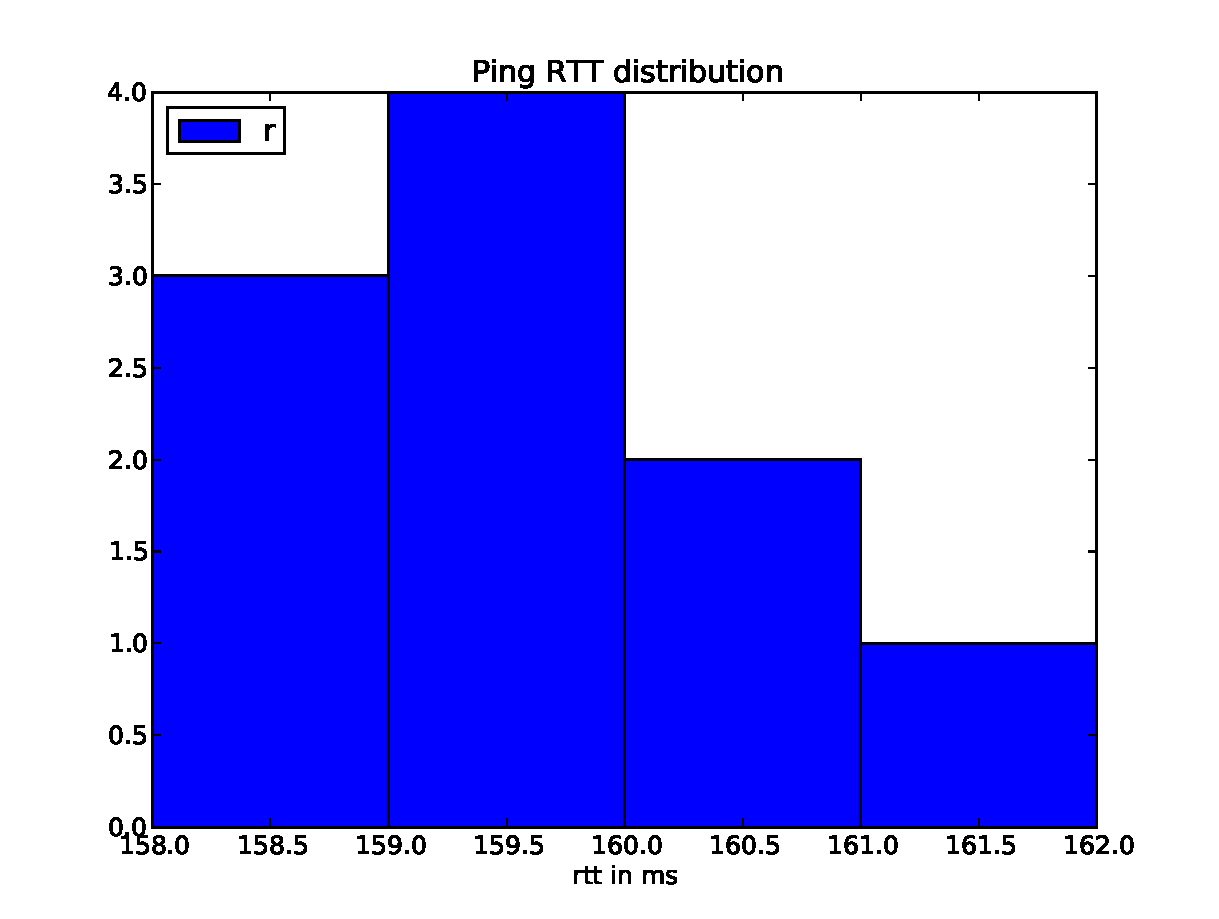
\includegraphics[height=6cm, width=7cm]{ping_distribution.pdf}  
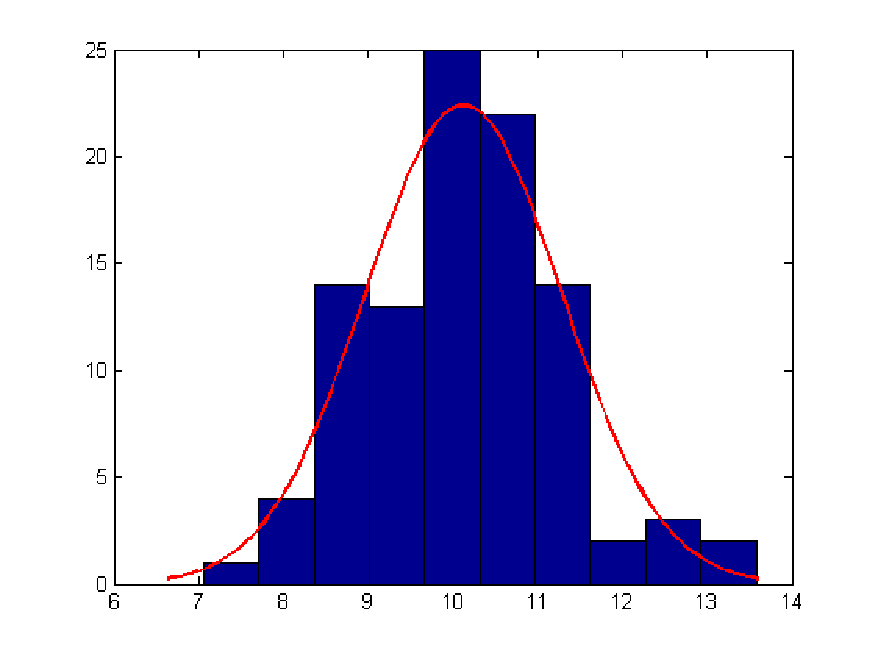
\includegraphics[height=5.5cm, width=7cm]{histo_gauss.pdf}
\end{columns}
\end{pyframe}

\subsection{Deviation}
\begin{pyframe}{Standard Deviation: scipy}
\begin{columns}
\column[t]{.4\textwidth}

\begin{itemize}
\item Standard deviation or $\sigma$ formula is {\large  $\sigma^{2}(X) := \frac{ \sum(x-\bar{x})^{2} }{n} $ }
\item $\sigma$ tells if $\delta$ is fair or not, and how much the mean ($\bar{x}$) is representative
\item \pymodule{matplotlib.mlab}.normpdf is a smooth function approximating the histogram
% Gauss function smoothly approximates the histogram {\Large 
%	$ \frac{n}{\sigma \sqrt{2\pi}}e^{-\frac{1}{2}  \big( \frac{x-\bar{x}} {\sigma} \big)^{2} } $ 
%} 
\end{itemize}

\column[t]{.6\textwidth}
\begin{pycode}
from scipy import std, mean
fair = [1, 1] # chickens
unfair = [0, 2] # chickens
assert mean(fair) == mean(unfair)

# Use standard deviation!
std(fair) # 0
std(unfair) # 1

\end{pycode}
\end{columns}
\end{pyframe}


\begin{pyframe}{Simple processing: scipy}
Check your computed values vs the $\sigma$ returned by ping 
(didn't you notice ping returned it?) 
\begin{pycode*}{escapeinside=||}
"""goal: remember to convert to numeric / float
   goal: use scipy
   goal: check stdev"""
from scipy import std, mean # max,min are builtin
rtt = ping_rtt()

print(max(rtt), min(rtt), mean(rtt), std(rtt))

\end{pycode*}
%fmt_s = 'stdev: {}, mean: {}, min: {}, max: {}'
%rtt_std, rtt_mean = |\pyver{std}|(rtt), |\emph{mean}|(ping_rtt)
%rtt_max, rtt_min = max(rtt), min(ping_rtt)
%print(fmt_s.format(rtt_std, rtt_mean, rtt_max, rtt_min))
\end{pyframe}

\begin{pyframe}{Time Distributions: Exercise}
\begin{itemize}
\item Parse the \href{https://github.com/ioggstream/python-course/blob/master/python-for-sysadmin/data/maillog}{provided maillog} in ipython using its ! magic and get an hourly email $\delta$
\item Expected output: 
\begin{pycode}
time_d = {  # mail delivered (removed) between
    0: xxx  #  00:00 - 00:59
    1: xxx  #  01:00 - 01:59
    ..
    }
\end{pycode}
\end{itemize}
\end{pyframe}
 
\iftrue
\begin{pyframe}{Time Distributions: Exercise Solution}
%def get_slot(ts):
%    n = int(ts[:2])
%    return n - (n%4)
\begin{pycode}
# deliveder emails are like the following 
#May 14 16:00:04 rpolli postfix/qmgr[122]: 4DC3DA: removed"
    
ret = !grep removed maillog # get the interesting lines

ts = ret.fields(2) # find the timestamp (3rd column)

hours = [ int(ts)  for x in ts ]
time_d = {x: count(x) for x in set(hours)}
\end{pycode}
\end{pyframe}

\fi 

\begin{pyframe}{Plotting distributions}
\begin{columns}
\column[t]{.6\textwidth}
\begin{pycode}
# To plot data..
from matplotlib import pyplot as plt
# and set the interactive mode
plt.ion()

# Plotting an histogram... 
frequency, bins, _ = hist(hours)

# .. returns a 
distribution = dict(zip(slots, 
    frequency))
\end{pycode}
\column[t]{.4\textwidth}
This server works mostly at night...
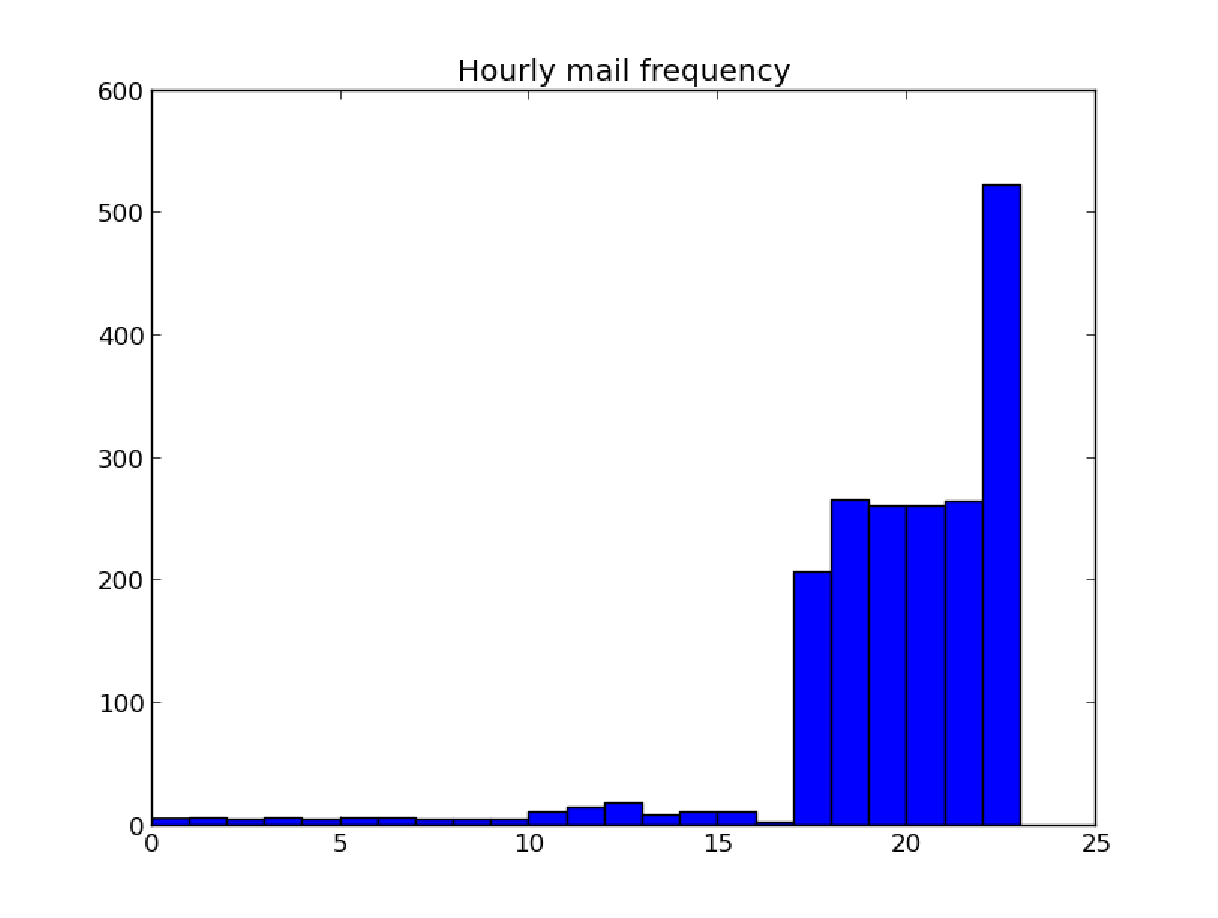
\includegraphics[width=6cm,height=5cm]{hourly_mail_d.pdf}
\end{columns}
\end{pyframe}

\begin{pyframe}{Size Distributions: Exercise}
\begin{itemize}
\item Create a size $\delta$ using \pyfunction{hist}(..., bins=...)
\item Hint: help(hist)
\begin{pycode}
size_d = {  # mail size between
    0: xxx  #  0 - 10k
    1: xxx  #  10k - 20k
    ..
    }
\end{pycode}
\item Homework: Use the size $\delta$ to find size\_mean and size\_sigma and compare with $\sigma$ and mean evaluated from the original data-series
\end{itemize}
\end{pyframe}



\begin{pyframe}{Simulating data with $\sigma$ and $\bar{x}$}
We can use  mean and a stdev to simulate data using the gaussian distribution.
This is obviously \emph{just a starting point}.
\begin{pycode*}{escapeinside=||}
from random import gauss
# In a mail load generator script we can simulate a
mail_size = int(gauss(mean, sigma_s))

# and use time_d to simulate the load during the day
from time import localtime
hour = localtime().tm_hour
hour = hour - (hour % 4)
mail_per_minute = time_d[hour] / |\pyver{(4 * 60)}| # minutes in 4hours
\end{pycode*}
\end{pyframe}



\subsection{Correlation}
\begin{pyframe}{Linear Correlation}
\begin{columns}
\column[t]{.6\textwidth}
\begin{pycode}
#Let's plot the following 
# datasets
mail_sent = [1, 5, 500, 250, 100, 7]
kB_s = [70, 300, 29000, 12500, 450, 500]

# A scatter plot can suggest relations 
#  between data
plt.scatter(mail_sent, kB_s)





\end{pycode}
\column[t]{.4\textwidth}
\footnotesize
Correlating Mail and Thruput
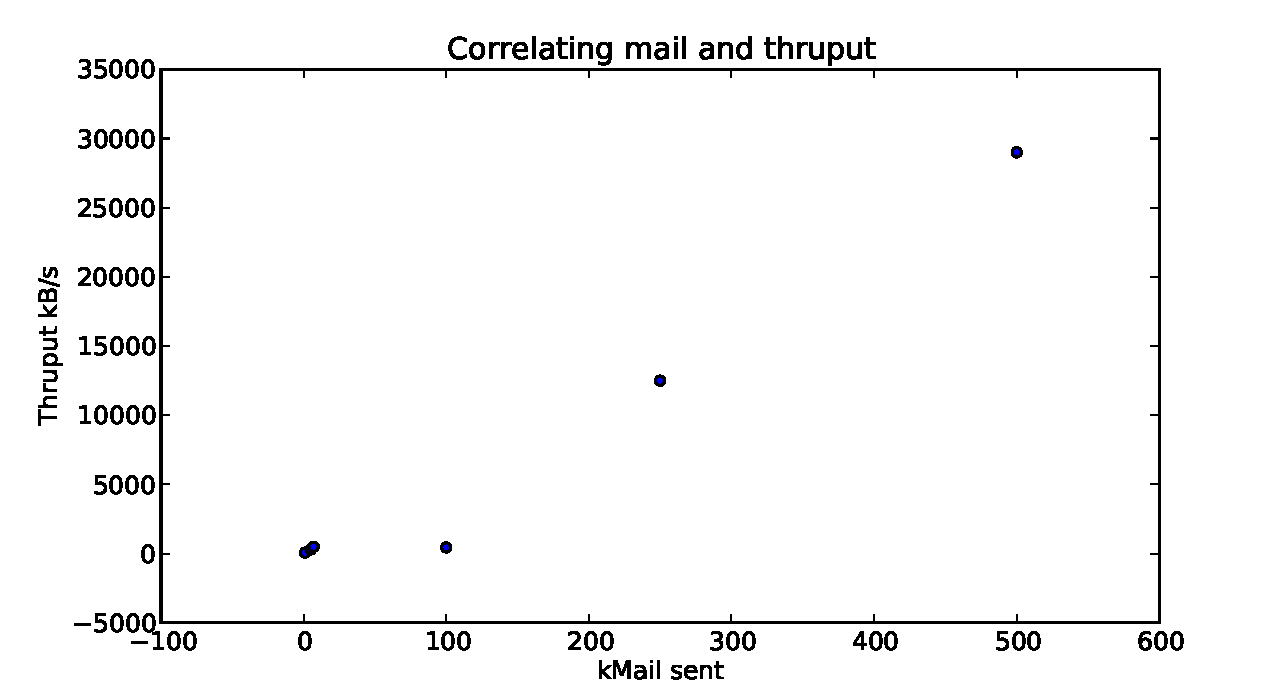
\includegraphics[height=5cm,width=7cm]{scatter_mail.pdf}
\end{columns}
\end{pyframe}


\begin{pyframe}{Linear Correlation}
The Pearson Coefficient is a relation indicator. 
\begin{description}
\item[0]  no relation
\item[1]  direct relation (both dataset increase together)
\item[-1]  inverse relation (one increase as the other decrease) 
\end{description}

\begin{pycode}
from scipy.stats.stats import pearsonr
ret = pearsonr(mail_sent, kB_s)
print(ret)
>(0.9823, 0.0004)
correlation, probability = ret
\end{pycode}
\end{pyframe}

\begin{pyframe}{You \emph{must (scatter) plot!}}
\LARGE
\begin{center}
PearsonR does not detect non-linear correlation \\
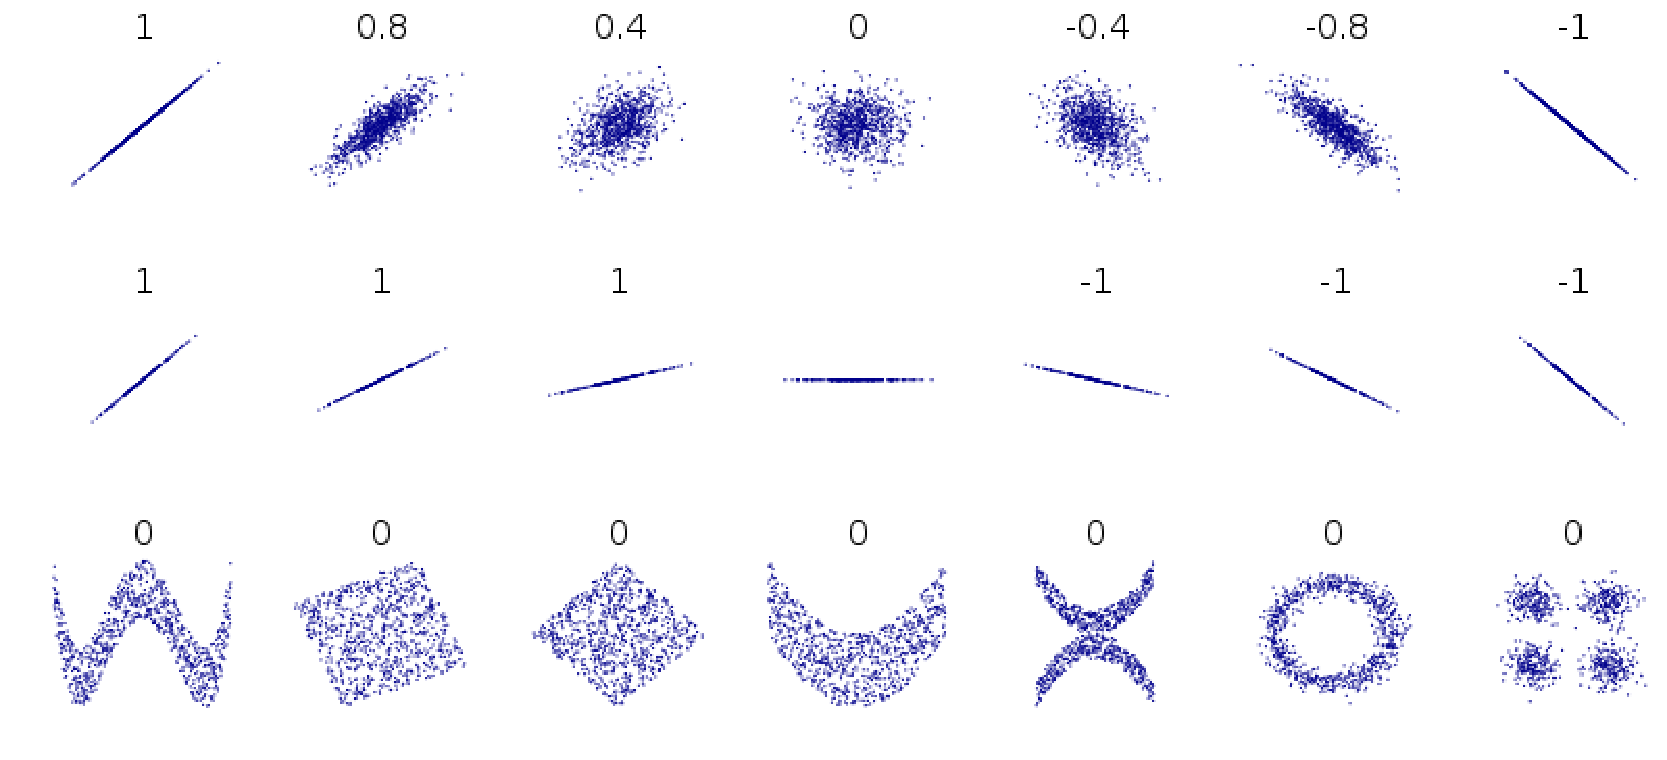
\includegraphics[width=.8\textwidth]{correlation.pdf} \\
\end{center}
\end{pyframe}


\begin{pyframe}{Combinations } % \dbinom{n}{k}}
\begin{columns}
\column[t]{.6\textwidth}
\begin{pycode}
# Given a table with many data series
from course import table
table = {...
  'cpu_usr': [10, 23, 55, ..],
  'byte_in': [2132, 3212, 3942, ..], }

# We can combine all their names with
from itertools import combinations
list(combinations(table,2))
>[('swap_in', 'cpu_sys'),
 ('swap_in', 'csw'),  ('cpu_sys', 'csw')... ]








\end{pycode}
\column[t]{.3\textwidth}
Combinating 4 suites, 2 at a time.
\hearts \spades \\
\hearts \clubs \\
\hearts \diamonds \\
\spades \clubs \\
\spades \diamonds \\
\clubs \diamonds \\


%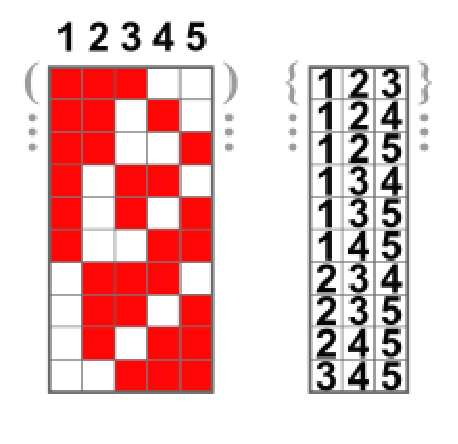
\includegraphics[width=4cm]{combinations_3.pdf}
\end{columns}
\end{pyframe}


\begin{pyframe}{Netfishing correlation}
We can try every combination between data series and check if there's some linear correlation.
\begin{pycode}
for k1, k2 in combinations(table, 2):
  corr, probability = pearsonr(table[k1], table[k2])
  if corr < 0.5:
    # I'm *still* not interested in data under this threshold
    continue
  print("linear correlation between {} and {} is {}".format(
    k1, k2, corr))

\end{pycode}
\end{pyframe}

\begin{pyframe}{Netfishing correlation II}
\begin{pycode}
from matplotlib import pyplot as plt
# create all combined plot
for k1, k2 in combinations(table, 2):
    corr, probability = pearsonr(table[k1], table[k2])
    plt.scatter(table[k1], table[k2])

    # 3 digit precision on title
    plt.title("R={:0.3f}".format(corr))
    plt.xlabel(k1); plt.ylabel(k2)

    # save and close the plot
    plt.savefig("{}_{}.png".format(k1, k2)); plt.close()
\end{pycode}
\end{pyframe}


\begin{pyframe}{Mark time with colors}
\begin{pycode*}{escapeinside=||}
# Use 6 colors to mark time-slots
from itertools import cycle
colors = cycle('rygcBm') # Red Green Blue ...

# then import a function to chunk datasets
from course import in_chunks

list(in_chunks(range(10), size=4)))
> [[0, 1, 2, 3], 
  [4, 5, 6, 7], 
  [8, 9]]
\end{pycode*}
\end{pyframe}

\begin{pyframe}{Mark time with colors}
\begin{pycode*}{escapeinside=||}
# Get combined data directly via $\pyver{items}$
#  TODO: add some plot figures of this section
for (k1, v1), (k2, v2) in combinations(table.|\pyver{items}|(), 2):
    corr, probability = pearsonr(v1, v2)

    # Two nice generators
    time_chunked = zip(in_chunks(v1, size=11), in_chunks(v2, size=11))
    [plt.scatter(t1, t2, color=next(colors)) 
        for t1, t2 in time_chunked]

    # save and close the plot
    plt.savefig("time_4h_{}_{}.png".format(k1, k2)); plt.close()
\end{pycode*}
\end{pyframe}

\section{End}
\begin{pyframe}{That's all folks!}
Thank you for the attention!
\end{pyframe}


